\section{\ExercisePrefixEmbeddedC Android Bluetooth Low Energy \optional}
ABLE (Android Bluetooth Low Energy) ist eine Applikation für Androidgeräte, um über BLE (Bluetooth Low Energy) eine drahtlose Verbindung zwischen einem Android Smartphone und einem anderen beliebigen BLE-Device herzustellen. Der Mikrocontroller des C/C++-Praktikums kann durch ein zusätzliches Modul, welches bereitgestellt wird, mit BLE erweitert werden. Du kannst auf einem Android Smartphone die ABLE Applikation installieren und dich mit dem Mikrocontroller verbinden. Abbildung \ref{fig:ablePreview} zeigt ein Beispielsprogramm indem der Mikrocontroller den X-Wert des Joystick 1 über BLE an ein Android Smartphone sendet. Eine ausführliche Anleitung zur Nutzung von ABLE auf dem Mikrocontroller des Praktikums findest du unter \href{https://github.com/Echtzeitsysteme/able/wiki/Cpp-Lab-Tutorial}{diesem Link [1]}. 
\begin{figure}[!htb]
	\centering
	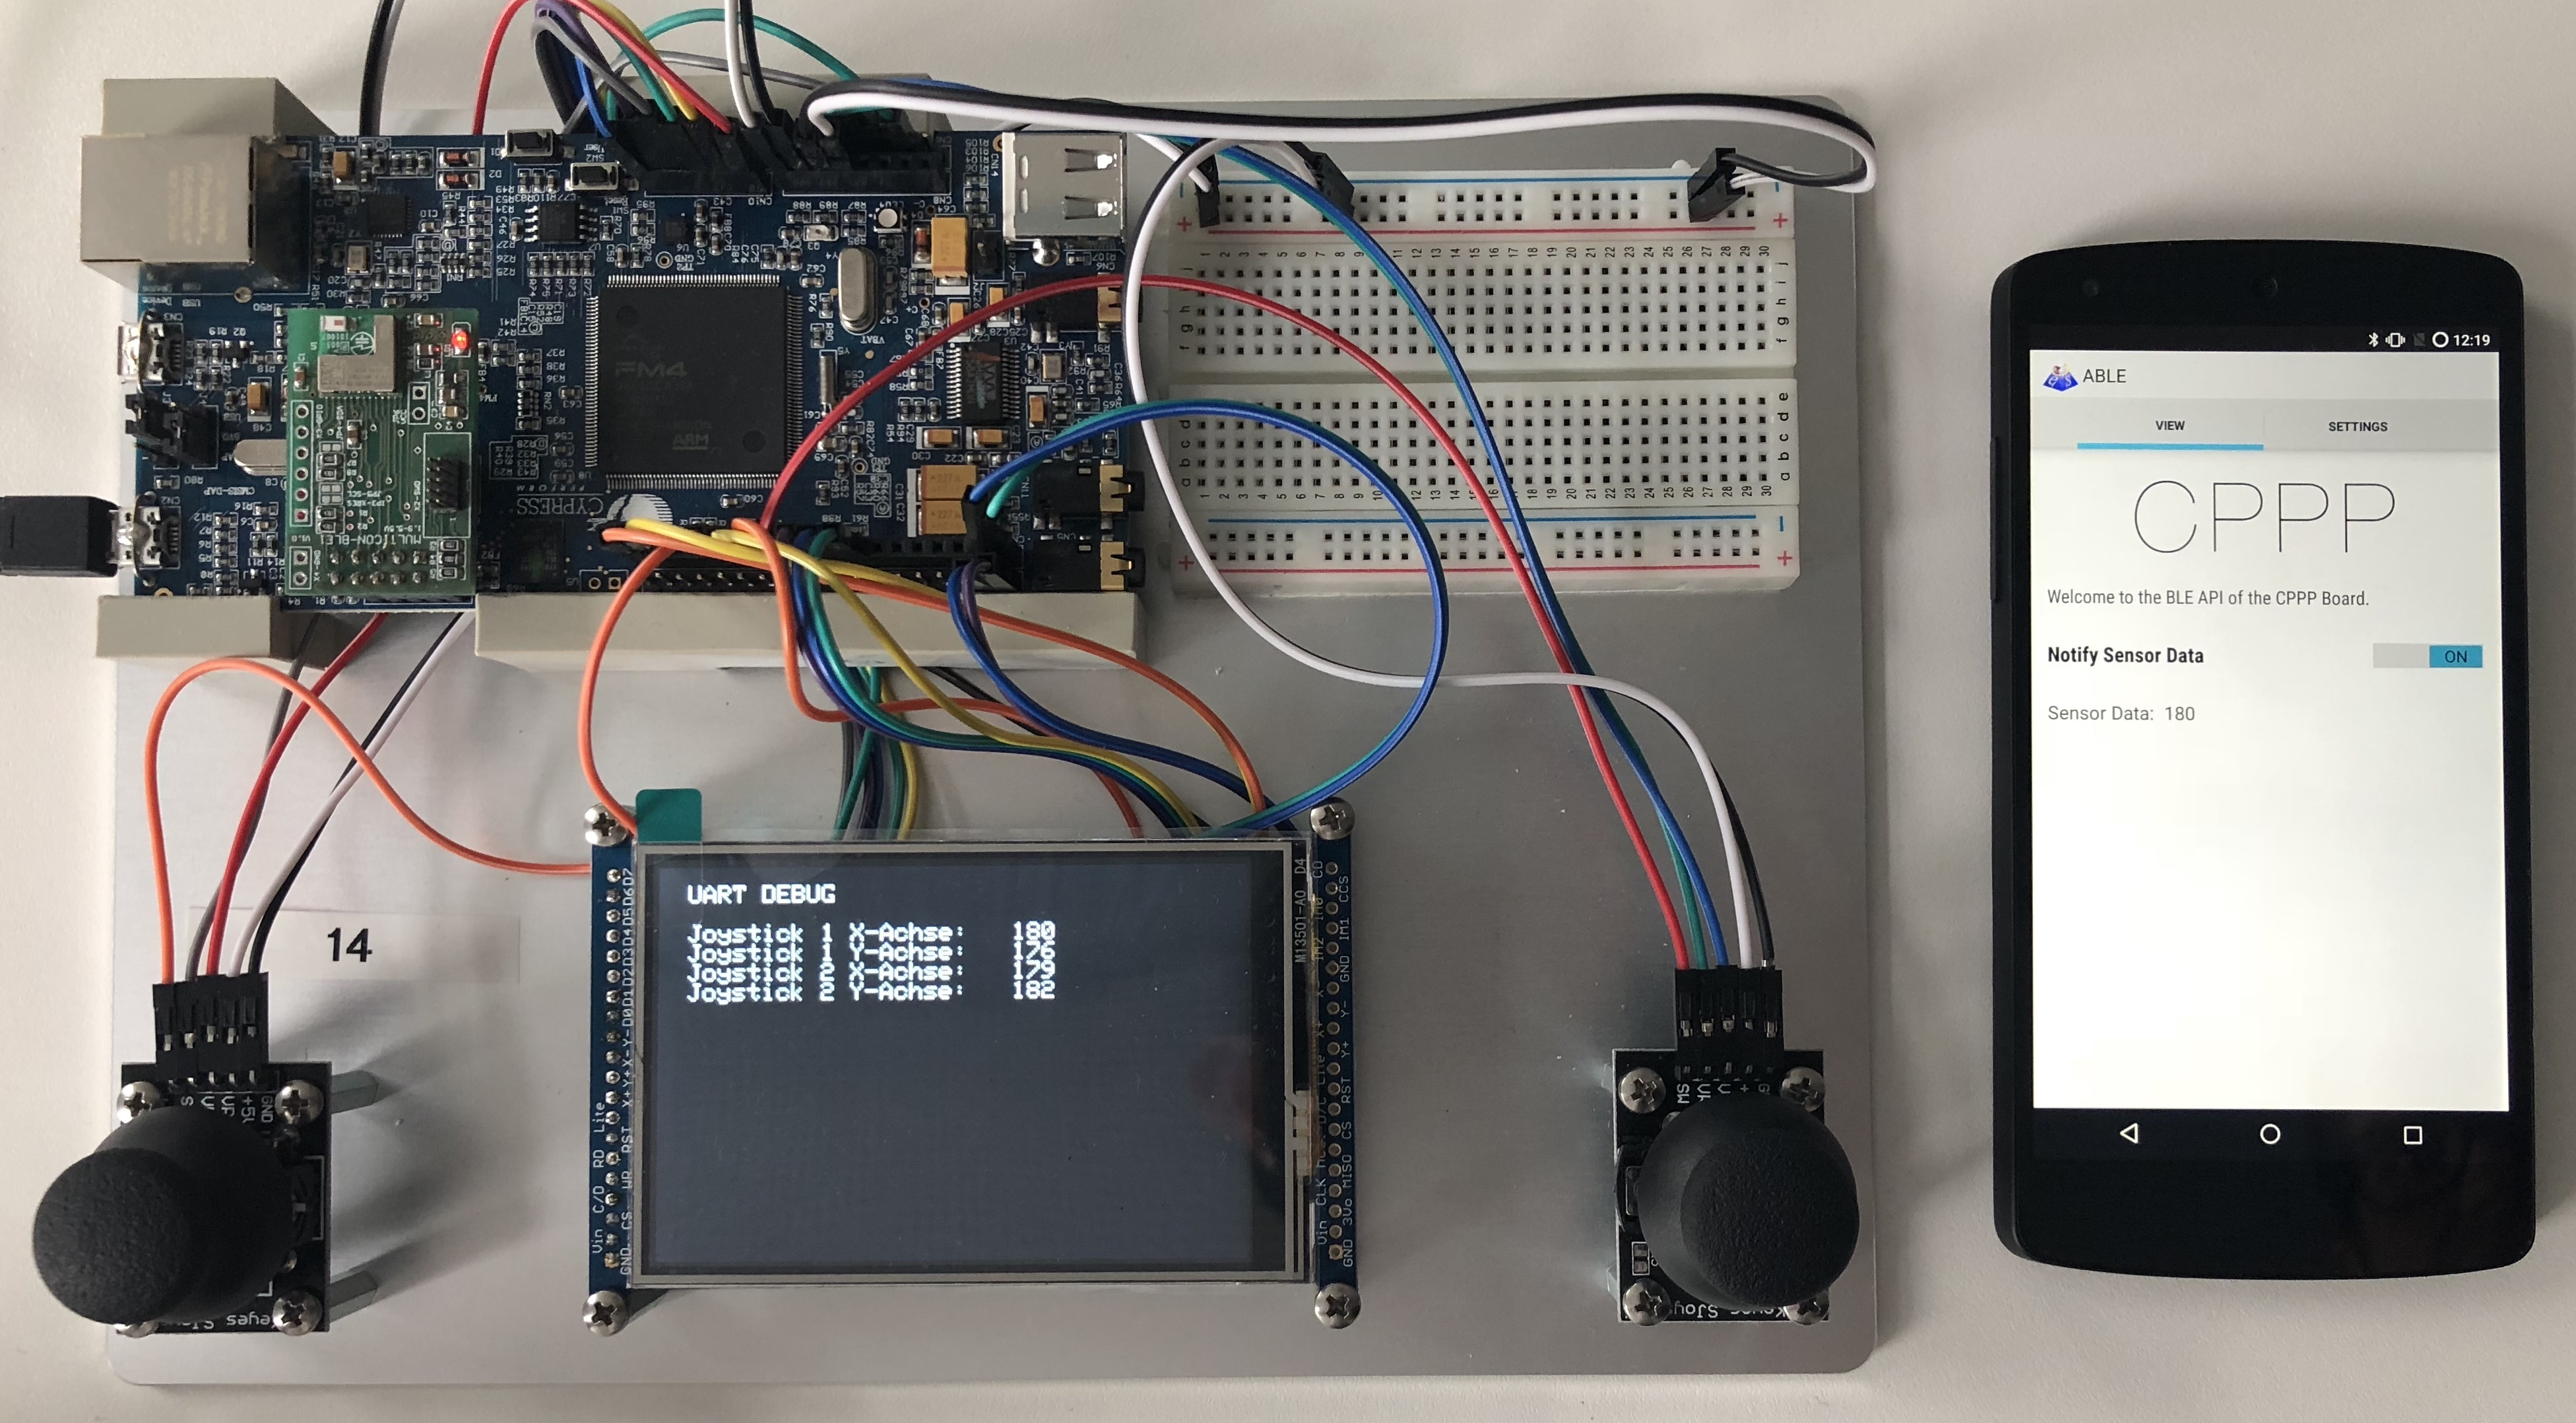
\includegraphics[width=0.7\textwidth]{./05_c/figures/ABLE_preview.jpg}
	\caption{Der C/C++-Mikrocontroller verbunden über Bluetooth mit einem Android Smartphone}
	\label{fig:ablePreview}
\end{figure} 
